\documentclass[10pt]{article}
\usepackage{icmlko}

\icmlmeta{IP 파운데이션 월드모델}{274}{재현되는 잡음}{쓰려던 $-$0.067 은 짝지어 재니 $+$0.007 이었다 --- 그런데 다른 변경 하나가 정확히 그 크기를 낸다}

\begin{document}

\twocolumn[
\icmlheader

\begin{abstract}
저장소에서 팝업(이 프로젝트가 시작된 도메인)의 걸음을 뽑았더니
\textbf{17축 $+$0.4287 $\to$ 23축 $+$0.3615} 였다. 웹툰 · 애니 \emph{전용}
축 여섯을 넣었는데 값이 한 자리도 안 바뀌는 팝업이 $-$0.067 을 냈다 ---
노트 258 · 259의 자리바꿈이 하필 출발점을 쳤다는 이야기가 된다. 논문을
거의 다 썼다. 그리고 \textbf{짝지어 다시 쟀더니 $+$0.0071 (t${=}$0.17)
이었다.} 세 실행을 가로질러 뺀 것이 틀렸다. 어디서 왔나 갈랐다 ---
저장된 17축 값은 07-30 16:29 것이고 노트 262 · 263이 그 뒤에 웹툰 두 열을
막았다. \textbf{축 세트 이름은 안 변했는데 그 이름이 가리키는 열이 변했다.}
그 마스킹만 따로 짝지어 재니 팝업 \textbf{$-$0.0690}(17축) ·
\textbf{$-$0.0528}(23축) --- \textbf{내가 쓰려던 수가 다른 원인으로
재현된다.} 그런데 이것도 진짜가 아니다: $t{=}{-}1.3$ 이고 \texttt{spread}
의 진짜 총량이 두 축 세트 다 \textbf{0.0000} 이다. 팝업의 짝 SE 가
0.040$\sim$0.053 으로 판에서 둘째로 나쁘기 때문이다. 여기서 일반 법칙
하나가 떨어진다 --- 도메인마다 \textbf{재면 보이는 크기}(2 짝SE)와
\textbf{판이 쓸 수 있는 크기}(0.010 $\div$ 몫)가 따로 있고, 아홉 중
\textbf{웹툰만} 뒤가 앞보다 작다. 팝업은 도메인 안에서 $\Delta\rho{=}0.435$
가 있어야 판이 겨우 본다. \textbf{팝업 전용 축은 안 팔리는 게 아니라 팔릴
수 없다.} 덤으로 하나 --- 노트 262 · 263의 새는 열 제거는 판에
$-$0.0096 · $-$0.0015 를 물렸고 둘 다 노트 245의 미결정 폭 안이다.
\textbf{누출을 뗀 값은 공짜였다.}
\end{abstract}
]

\section{거의 다 쓴 논문}

노트 273이 저장소(\texttt{data/lab/lab.db})를 열게 만들었다. 새로 적합할
필요 없이 물음 하나를 답할 수 있어 보였다 --- 축을 다섯에서 스물셋으로
늘리는 동안 팝업은 어떻게 됐나.

\begin{center}\small
\begin{tabular}{lrr}
\hline
축 세트 & 축 & 저장된 팝업 \\
\hline
base & 5 & $+$0.2805 \\
trendcalwiki & 17 & $+$0.4287 \\
$+$태그 · 메타 & 23 & $+$0.3615 \\
\hline
\end{tabular}
\end{center}

$-$0.067 이다. 그리고 그 축 여섯은 \texttt{tag\_c1\_웹툰} 처럼 \textbf{웹툰 ·
애니 전용}이라 팝업 행에서는 마스크 0 이다. 팝업의 입력이 한 비트도 안
바뀌었는데 점수가 내린다 --- 노트 259가 잰 기전(쓸모 있는 열은 뿌리 근처에서
갈리고, 그 분기는 아홉 도메인이 함께 내려가는 길이다)이 하필 이 프로젝트의
출발점을 쳤다는 이야기다.

제목까지 붙였다. 그런데 그 셋이 서로 다른 실행이라, 노트 248이 잰 팝업의
짝 SE 를 생각하면 2 SE 언저리였다. 그래서 \textbf{같은 씨앗으로 짝지어 다시
쟀다.}

\begin{figure*}[t]
\centering
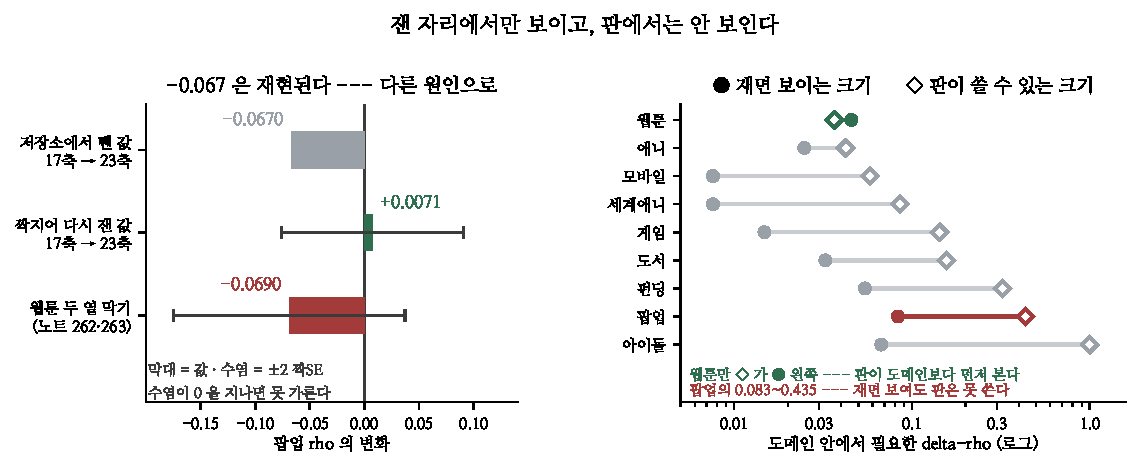
\includegraphics[width=\textwidth]{figs/popup.pdf}
\caption{왼쪽 --- 크기가 같은 수 셋. 저장소에서 뺀 $-$0.067, 짝지어 잰
$+$0.0071, 웹툰 두 열을 막아서 나온 $-$0.0690. 수염이 0 을 지나므로 뒤의
둘은 못 가른다. 오른쪽 --- 도메인마다 ● 재면 보이는 크기(2 짝SE)와
◇ 판이 쓸 수 있는 크기(0.010 $\div$ 몫). 아홉 중 웹툰만 ◇ 가 ● 왼쪽에
있다.}
\end{figure*}

\section{$+$0.0071}

\begin{center}\small
\begin{tabular}{lrrrr}
\hline
도메인 & 17축 & 23축 & 차 & $t$ \\
\hline
웹툰 & 0.3114 & 0.4533 & $+$0.1419 & 6.22 \\
애니 & 0.4658 & 0.5047 & $+$0.0389 & 3.13 \\
\textbf{팝업} & 0.3544 & 0.3614 & \textbf{$+$0.0071} & \textbf{0.17} \\
게임 & 0.6189 & 0.6221 & $+$0.0032 & 0.43 \\
세계애니 & 0.5349 & 0.5343 & $-$0.0006 & $-$0.14 \\
모바일 & 0.5389 & 0.5353 & $-$0.0036 & $-$0.97 \\
아이돌 & 0.1476 & 0.1370 & $-$0.0106 & $-$0.32 \\
도서 & 0.3856 & 0.3689 & $-$0.0167 & $-$1.03 \\
펀딩 & 0.2972 & 0.2674 & $-$0.0298 & $-$1.10 \\
\hline
판 & 0.4384 & 0.4845 & $+$0.0461 & \\
\hline
\end{tabular}
\end{center}

\textbf{팝업은 안 잃었다.} 축을 받은 둘만 오르고($t{=}6.22$ · $3.13$)
나머지 일곱은 다섯이 음수 · 둘이 양수인데 \textbf{$|t|$ 가 전부 1.1 아래}다.
자리바꿈은 부호로는 살아 있지만 크기가 0.01$\sim$0.03 이고 어느 한
도메인에 몰리지도 않는다. \textbf{제일 많이 잃은 것은 팝업이 아니라
펀딩($-$0.0298)이다.}

노트 133이 첫 양수를 그대로 채택하지 말라고 했다. 이번엔 첫 \emph{음수}였다.

\section{그러면 $-$0.067 은 어디서 왔나}

버리기 전에 갈랐다. 저장소에서 F18 의 팝업 배포 점수를 시각과 함께
꺼냈다.

\begin{center}\small
\begin{tabular}{llr}
\hline
시각 & 형식 & 팝업 \\
\hline
07-30 15:08 & \texttt{@trendcalwiki} & $+$0.4305 \\
07-30 15:18 & \texttt{@trendcalwiki} & $+$0.4305 \\
07-30 16:29 & \texttt{@trendcalwiki} & $+$0.4287 \\
07-31 15:07 & \texttt{@trendcalwikitag} & $+$0.3615 \\
07-31 15:24 & \texttt{@trendcalwikitag} & $+$0.3615 \\
\hline
오늘 짝 & \texttt{@trendcalwiki} & \textbf{$+$0.3544} \\
오늘 짝 & \texttt{@trendcalwikitag} & $+$0.3614 \\
\hline
\end{tabular}
\end{center}

\textbf{23축은 정확히 재현된다}(0.3615 대 0.3614). \textbf{17축은 안 된다}
--- 07-30 에 0.4287$\sim$0.4305, 오늘 0.3544. 차이 0.075.

그 사이에 무엇이 있었나. \textbf{노트 262(07-31 13:55)와 노트
263(14:01)}이다. 둘은 웹툰의 \texttt{entry\_friction} 이 사실
\texttt{daily\_pass} 고 \texttt{goods\_scale} 이 \texttt{n\_episode} 라는
것을 밝히고 \texttt{fixaxes.BLOCK} 으로 두 열의 마스크를 0 으로 내렸다.
\textbf{그 두 열은 손 축이라 모든 축 세트에 들어 있다} --- base 에도,
trendcalwiki 에도.

\begin{quote}\small
축 세트 이름(\texttt{trendcalwiki})은 안 변했다. 그 이름이 가리키는 열이
변했다. 저장소는 이름만 적는다.
\end{quote}

\section{정확히 그 크기가 나온다}

마스킹만 따로 짝지어 껐다 켰다.

\begin{center}\small
\begin{tabular}{lrrr}
\hline
& 막기 전 & 막은 뒤 & 차 \\
\hline
\multicolumn{4}{l}{\emph{17축}} \\
\textbf{팝업} & 0.4234 & 0.3544 & \textbf{$-$0.0690} \\
웹툰 & 0.3490 & 0.3114 & $-$0.0376 \\
도서 & 0.3410 & 0.3856 & $+$0.0447 \\
아이돌 & 0.0987 & 0.1476 & $+$0.0489 \\
판 & 0.4480 & 0.4384 & $-$0.0096 \\
\hline
\multicolumn{4}{l}{\emph{23축}} \\
\textbf{팝업} & 0.4142 & 0.3614 & \textbf{$-$0.0528} \\
웹툰 & 0.4782 & 0.4533 & $-$0.0249 \\
도서 & 0.3158 & 0.3689 & $+$0.0531 \\
아이돌 & 0.0770 & 0.1370 & $+$0.0600 \\
판 & 0.4860 & 0.4845 & $-$0.0015 \\
\hline
\end{tabular}
\end{center}

\textbf{$-$0.0690.} 내가 쓰려던 $-$0.067 이 소수점 둘째 자리까지 나온다 ---
\emph{다른 원인으로}. 게다가 방향까지 이야기에 맞는다: 웹툰 전용 열을
건드렸는데 팝업이 제일 많이 움직인다.

\textbf{그런데 이것도 진짜가 아니다.} $t{=}{-}1.3$(17축) ·
$-$1.33(23축)이고, \texttt{rank.spread} 의 \emph{진짜 총량}이 두 축 세트 다
\textbf{0.0000 · 진짜 0개}다. 팝업의 짝 SE 가 0.053 · 0.040 이라 $-$0.069
는 수염 안에 들어앉는다.

\paragraph{그러니까} 같은 크기의 수 셋을 봤다 --- 저장소에서 뺀
$-$0.067, 짝지어 잰 $+$0.0071, 마스킹이 낸 $-$0.0690. \textbf{셋 중 진짜는
없다.} 팝업에서는 이 크기가 전부 잡음이다.

\section{보이는 크기와 쓸 수 있는 크기}

왜 팝업에서만 이러나. 짝 SE 를 도메인별로 놓고, 노트 245가 정한 판의
미결정 폭 0.010 을 몫으로 나눠 봤다.

\begin{center}\small
\begin{tabular}{lrrrr}
\hline
도메인 & 몫 & 짝SE & 보이려면 & 판이 쓰려면 \\
\hline
웹툰 & 27.3\% & 0.0228 & 0.046 & \textbf{0.037} \\
애니 & 23.6\% & 0.0124 & 0.025 & 0.042 \\
모바일 & 17.2\% & 0.0038 & 0.008 & 0.058 \\
세계애니 & 11.7\% & 0.0038 & 0.008 & 0.085 \\
게임 & 7.0\% & 0.0074 & 0.015 & 0.143 \\
도서 & 6.4\% & 0.0163 & 0.033 & 0.156 \\
펀딩 & 3.1\% & 0.0272 & 0.054 & 0.323 \\
\textbf{팝업} & 2.3\% & 0.0417 & 0.083 & \textbf{0.435} \\
아이돌 & 1.0\% & 0.0336 & 0.067 & 1.000 \\
\hline
\end{tabular}
\end{center}

\textbf{아홉 중 웹툰만 ``판이 쓰려면''이 ``보이려면''보다 작다.} 웹툰은
도메인 안에서 확인되기 \emph{전에} 판이 먼저 반응한다. 나머지 여덟은
반대다 --- \textbf{도메인 안에서는 뚜렷이 보이는데 판은 끝내 못 쓰는 구간이
있다.} 팝업에서 그 구간은 0.083 부터 0.435 까지고, 이 실험실이 지금까지
한 도메인에 그만큼 실은 변경은 웹툰 제 축(+0.1419) 하나뿐이다.

그래서 노트 274의 ``남은 것''에 적었던 \textbf{팝업 전용 축}은 다시 봐야
한다. 팝업 프로젝트 레코드 380건에는 아직 축이 아닌 열이 남아 있다 ---
\texttt{competition.*} 넷과 \texttt{calendar.*} 넷이 덮음 100\%,
\texttt{duration.*} 셋이 97\% 인데, 지금 쓰는 손 속성 일곱은 덮음 25\% 다.
\textbf{그 열들로 팝업을 올려도 판은 못 본다.} 올릴 이유는 여전히 있다 ---
노트 254가 적은 대로 판정 단위와 배포 단위는 다르고 도구를 팝업에 쓰는
사람에게는 실제 개선이다. 다만 \textbf{순위로는 결재가 안 난다}는 것을
이제 숫자로 안다.

\section{덤 --- 누출을 뗀 값}

노트 262 · 263은 새는 열 둘을 막았고, 위 표에서 그 대가는 판
$-$0.0096(17축) · $-$0.0015(23축)다. \textbf{둘 다 노트 245의 미결정 폭
0.010 안이다.} 누출을 떼는 데 잴 수 있는 값을 안 치렀다.

(노트 262 · 263은 그때 판을 .4916 $\to$ .4772 $\to$ .4842 로 적었다. 오늘의
0.4480 $\to$ 0.4384 와 안 맞는다. \textbf{맞을 수가 없다} --- 그 사이에
또 열이 변했다. 그게 이 노트의 요지다.)

\paragraph{남은 것}
\begin{center}\small
\begin{tabular}{ll}
\hline
갈래 & 왜 \\
\hline
문턱 40 대 15 & 팝업만 영향인데 팝업은 못 잰다. 판으로 \\
저장된 점수 & 이름이 같아도 못 뺀다. 시각을 적을까 \\
펀딩 $-$0.0298 & 제일 많이 잃었다. $t{=}{-}1.1$ 이라 더 봐야 \\
도메인별 배포 & 노트 254 · 이 노트가 두 번 짚었다 \\
\hline
\end{tabular}
\end{center}

\paragraph{규약} \textbf{저장된 도메인 점수는 실행을 가로질러 빼지 않는다.}
축 세트 이름은 안 변해도 그 이름이 가리키는 열은 변한다. 그리고 \textbf{수가
재현된다고 진짜인 것이 아니다} --- 이번에 $-$0.067 이 다른 원인으로 정확히
재현됐고, 둘 다 잡음이었다. 노트 253 · 259 · 261 · 267 · 270 · 273의 한
줄짜리 검정에 일곱 번째를 붙인다: \textbf{짝지어 재기 전에는 도메인 점수의
차를 안 믿는다.}

\end{document}
